% include the figures path relative to the master file
\graphicspath{{./content/experiments/figures/}}

\begin{figure}
  \centering
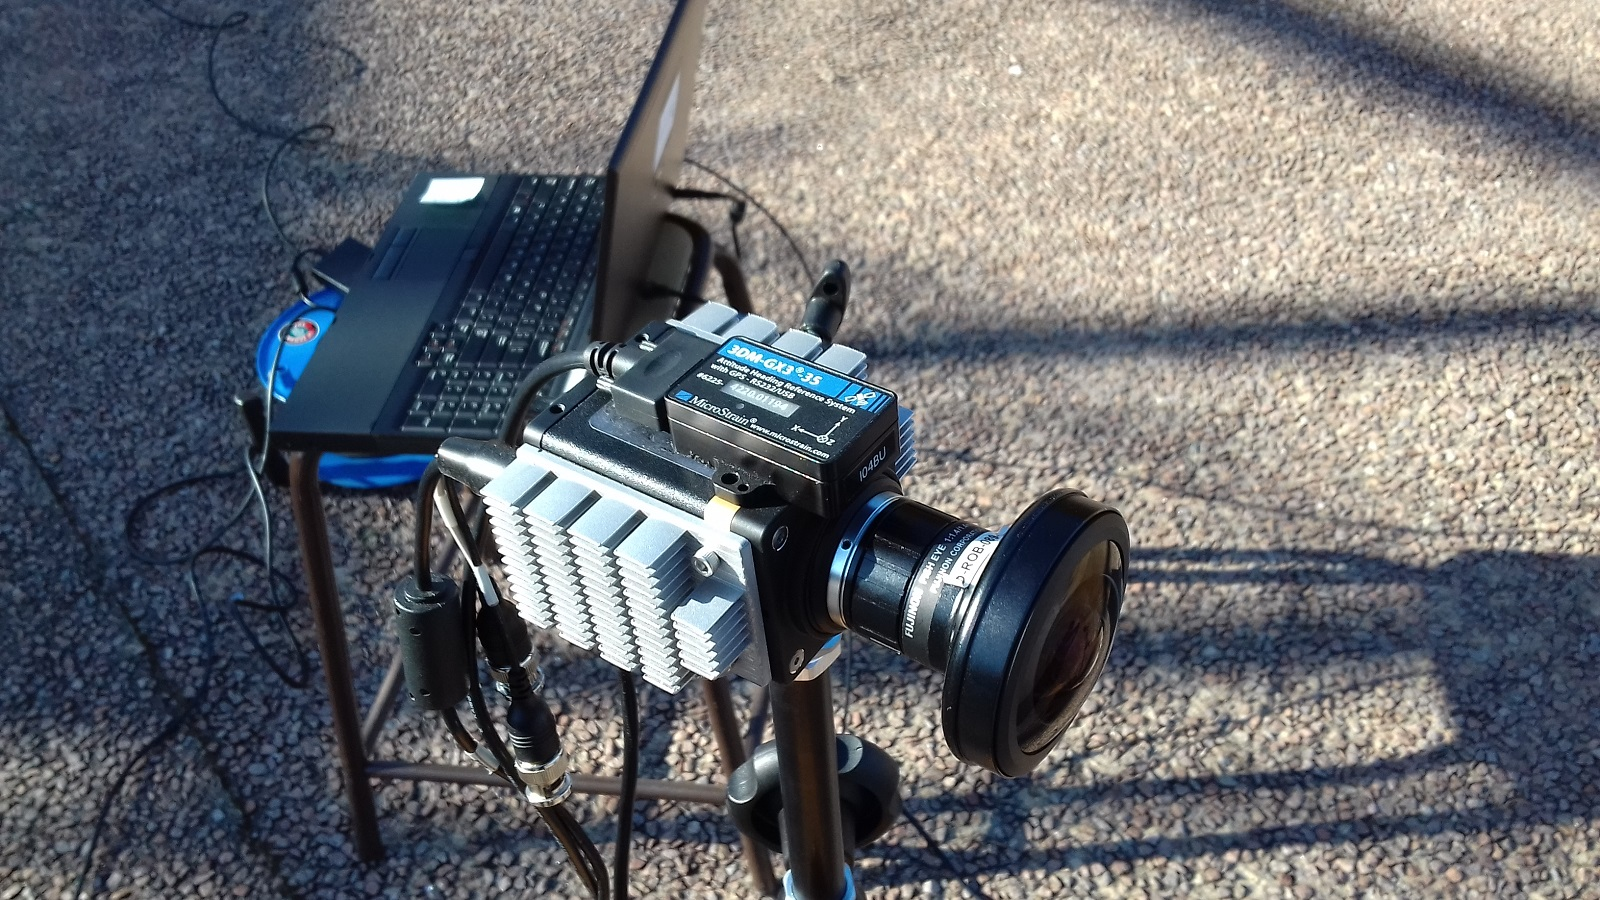
\includegraphics[width=0.33\textwidth]{./content/experiments/figures/setup.jpg}
\caption{Experimental setup.}
\label{fig:setup}
\end{figure}

\begin{figure*}
  \centering
  \subfigure[\gls{aop}]{\label{fig:aop-syn}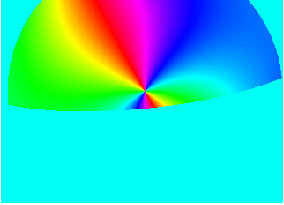
\includegraphics[width= 0.22\textwidth, height=0.12
    \textheight]{./content/experiments/figures/aop-no-noise.jpg}}\hfill
  \subfigure[\gls{dopl}]{\label{fig:dop-syn}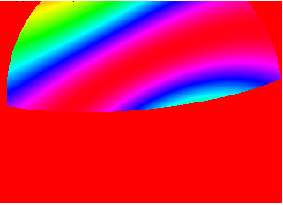
\includegraphics[width=0.22\textwidth, height=0.12
    \textheight]{./content/experiments/figures/dop-no-noise.jpg}}
  \hspace*{\fill}
  \subfigure[\gls{aop}]{\label{fig:aop-noisy-syn}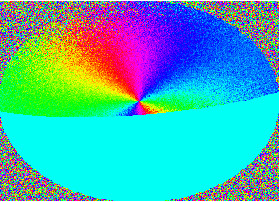
\includegraphics[width=0.22\textwidth,
    height=0.12\textheight]{./content/experiments/figures/aop-noise-01-2.jpg}
    }\hfill
  \subfigure[\gls{dopl}]{\label{fig:dop-noisy-syn}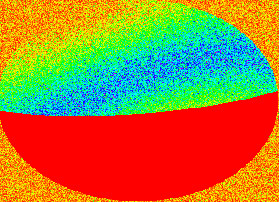
\includegraphics[width=0.22\textwidth,
    height=0.12\textheight]{./content/experiments/figures/dop-noise-01-2.jpg}
    }
  \hspace*{\fill}
  \caption{\gls{aop} and \gls{dopl} images synthetically created. All images
    have been generated with sky region for yaw, pitch and roll angle of
    \SI{1.8}{\radian}, \SI{-0.2}{\radian} and \SI{0.1}{\radian},
    respectively. (a)-(b) No noise added, (c)-(d) Noise level of 0.1 added.}
  \label{fig:aop-dop-syn}
\end{figure*}

\begin{figure*}
  \centering
  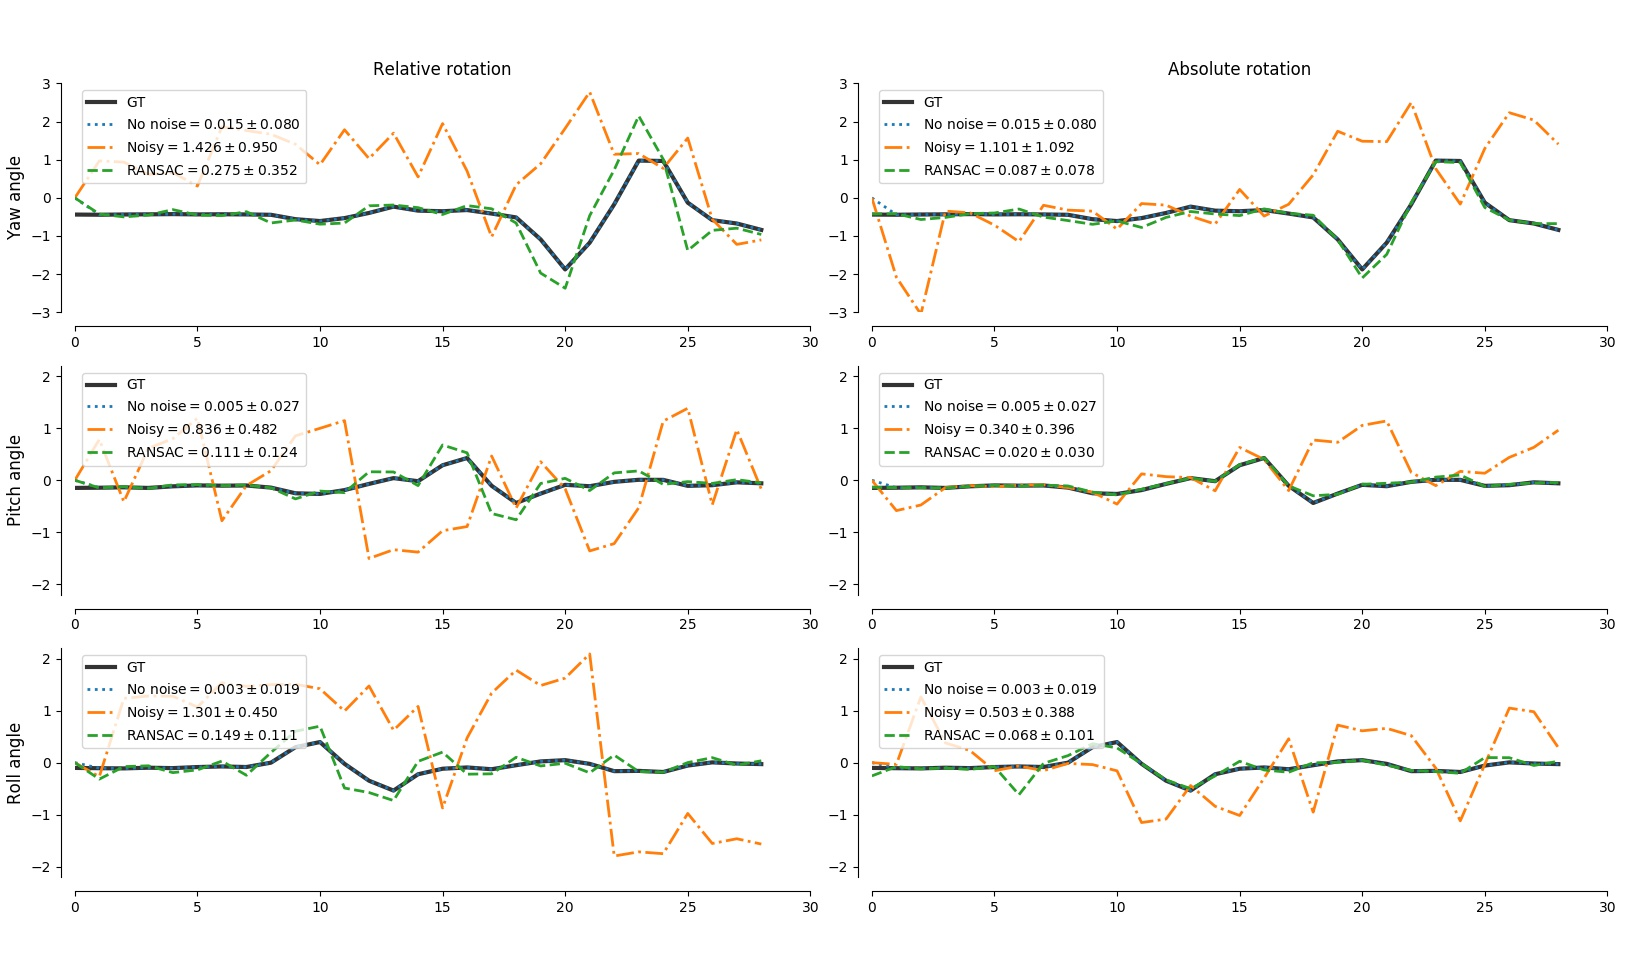
\includegraphics[width=1\textwidth]{./content/experiments/figures/syn-res.jpeg}
  \caption{Absolute and relative rotation obtained from synthetic data in ideal
  case, noisy conditions without RANSAC optimization and noisy case with RANSAC
optimization. The mean and standard deviation of the difference between each
predicted and \gls{gt} is illustrated in the legend as well.}
  \label{fig:res-syn}
\end{figure*}

\begin{figure}
  \centering
  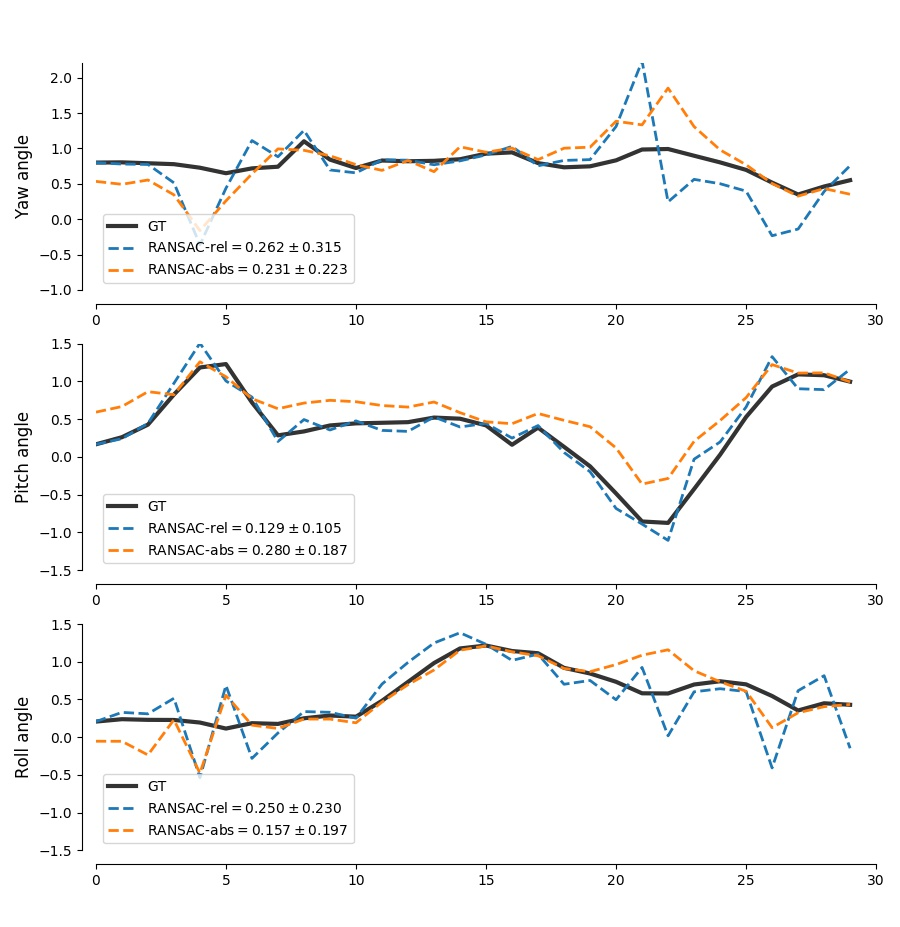
\includegraphics[width=0.49\textwidth]{./content/experiments/figures/real-res.jpeg}
  \caption{Absolute and relative rotation obtained from real data. The black
    line represents the \gls{gt}, the orange line and the blue line represent
    the absolute and relative predicted rotations, respectively.}
  \label{fig:res-real}
\end{figure}


\section{Experiments and Results}
\label{sec:exp-res}

This section presents our experimental setup, the designed experiments and the
obtained results. The setup used in our experiment is illustrated in
Fig.\,\ref{fig:rotation}. Instead of using a \gls{uav}, a camera was manually
moved (see Fig.\,\ref{fig:setup}). The \gls{imu} was calibrated with the camera
using \emph{kalibr} toolbox~\cite{furgale2013unified, furgale2012continuous},
to use the recordings as \gls{gt}. The polarimetric camera with fisheye lens
was also calibrated according to~\cite{kannala2006generic}.
Using the above setup two data sets of synthetic and real images were created
and the results obtained are presented in Exp.\,\ref{sec:exp1} and
Exp.\,\ref{sec:exp2}, respectively.

\subsection{Experiment~1}
\label{sec:exp1}
The synthetic data containing \gls{aop} and \gls{dopl} images of sky regions
were created using the \gls{imu} recordings obtained during real acquisition.
Figures~\ref{fig:aop-syn}~\&~\ref{fig:dop-syn} show an example of this dataset
at optimal conditions. This dataset based on \gls{imu} recordings contains
rotations along roll, pitch, and yaw. This dataset has originally 856 samples
but has been down-sampled by sampling rate of 30 samples.


Applying our framework on ideal synthetic data, perfect results were obtained
for absolute and relative rotations, while $\gamma$ was estimated using only 2
random points from the sky region (blue dotted curve in
Fig.\,\ref{fig:res-syn}).


% \begin{figure}
%   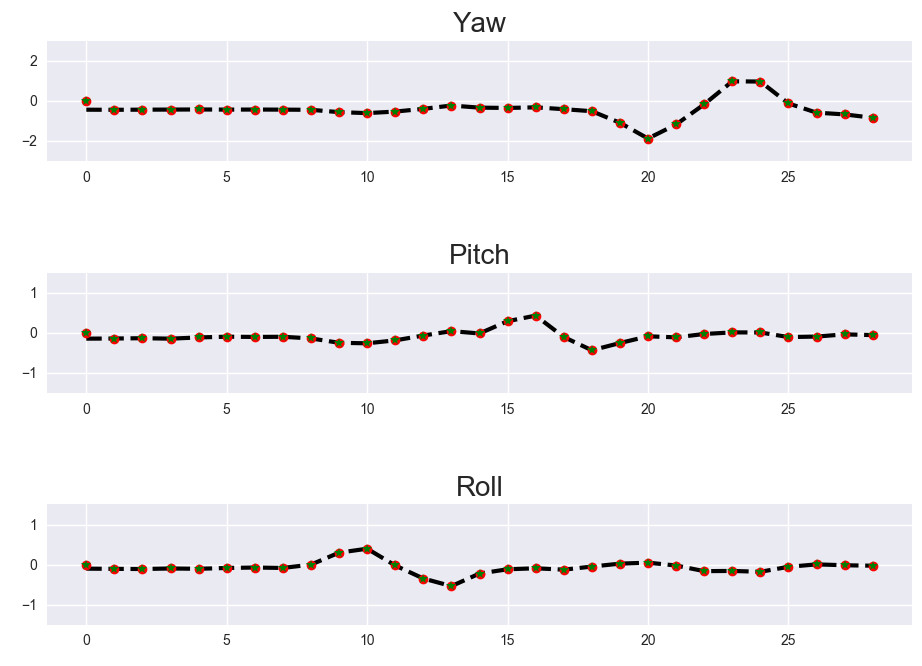
\includegraphics[width=0.47\textwidth]{./content/experiments/figures/ideal-syn-abs-rel-2.jpg}
%   \caption{Absolute and relative rotation obtained from synthetic data in
%     optimal conditions. The black line represents the \gls{gt}, the
%     \textcolor{red}{dots} and the \textcolor{green}{stars} represent the
%     absolute and relative predicted rotations, respectively.}
%   \label{fig:res-syn-ideal-abs-rel}
% \end{figure}

Although using our proposed framework, we were able to achieve perfect results
on ideal synthetic data, in reality it is rare to obtain the perfect skylight
polarization pattern. Variety of causes clutter the desired skylight pattern,
the main one being pollution. To account for such cases, a second test was
performed while significant level of noise was added to the created synthetic
data. Figures~\ref{fig:aop-noisy-syn}~\&~\ref{fig:dop-noisy-syn} show an
example of synthetic data with an additional Gaussian noise with an
standard-deviation of $0.1$.

% \begin{figure}
%   \centering
%   \subfigure[\gls{aop}]{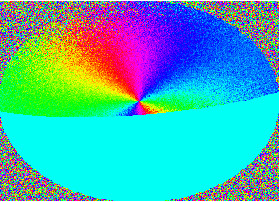
\includegraphics[width=0.22\textwidth,
%     height=0.12\textheight]{./content/experiments/figures/aop-noise-01-2.jpg}
%     \label{fig:aop-noise-syn}}\hfill
%   \subfigure[\gls{dopl}]{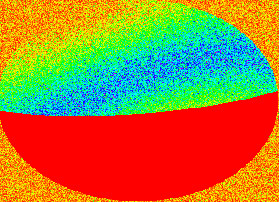
\includegraphics[width=0.22\textwidth,
%     height=0.12\textheight]{./content/experiments/figures/dop-noise-01-2.jpg}
%     \label{fig:dop-noise-syn}}
%   \hspace*{\fill}
%   \caption{Synthetically created \gls{aop} and \gls{dopl} images of sky
%       region with noise level of $0.1$. With yaw, pitch and roll angle of 1.8, -0.2 and 0.1, respectively.}
%   \label{fig:aop-dop-syn-noisy}
% \end{figure}

Performing the same 2 random-points algorithm as before on noisy dataset leads
to the results illustrated in Fig.\,\ref{fig:res-syn}, the orange curve. As
expected the performance decline, simply due to the noise.

% \begin{figure}
%   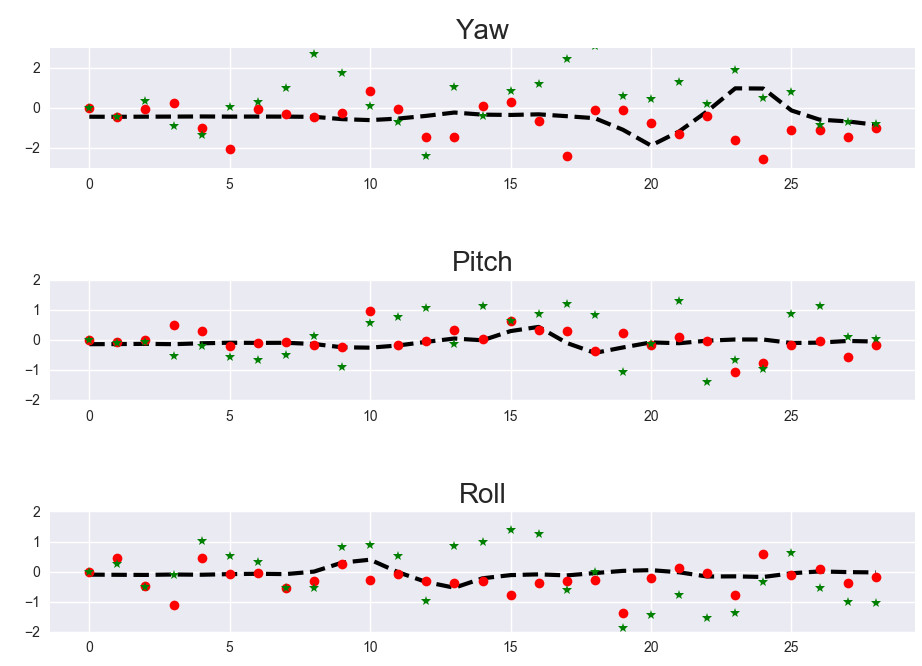
\includegraphics[width=0.5\textwidth]{./content/experiments/figures/noisy-syn-abs-rel-2.jpg}
%   \caption{Absolute and relative rotation obtained from synthetic data with
%     $10\%$ noise. The black line represents the \gls{gt}, the
%     \textcolor{red}{dots} and the \textcolor{green}{stars} represent the
%     absolute and relative predicted rotations, respectively.}
%   \label{fig:res-noisy-syn-abs-rel}
% \end{figure}

To solve this problem, \gls{ransac} was used to estimate the attitude in the
absolute and relative rotation methods. For the absolute rotation, since the
sun position is assumed to be known the model optimizes the full rotation of
each frame in comparison with the origin considering the difference between the
predicted and real sun positions.

However, in the relative rotation method there is no information about the
original position, or sun position, and the algorithm only depends on the
polarized vector, $v = R_{cp} . v_p$ between two different frames. Therefore,
using the model infers the optimal vector representing each frame is
obtained.

Estimating the attitude on the noisy dataset with \gls{ransac} significantly
improved the results as shown in Fig.\,\ref{fig:res-syn} (green-dashed
line). The parameters used were: an error threshold of 0.07, 10 random points
(2 points for defining the model and the rest as test), and 2000 iterations.
%the following results are obtained:
% \begin{figure*}
%   \centering
%   \subfigure[The theoretical method without \gls{ransac} optimization]{
%     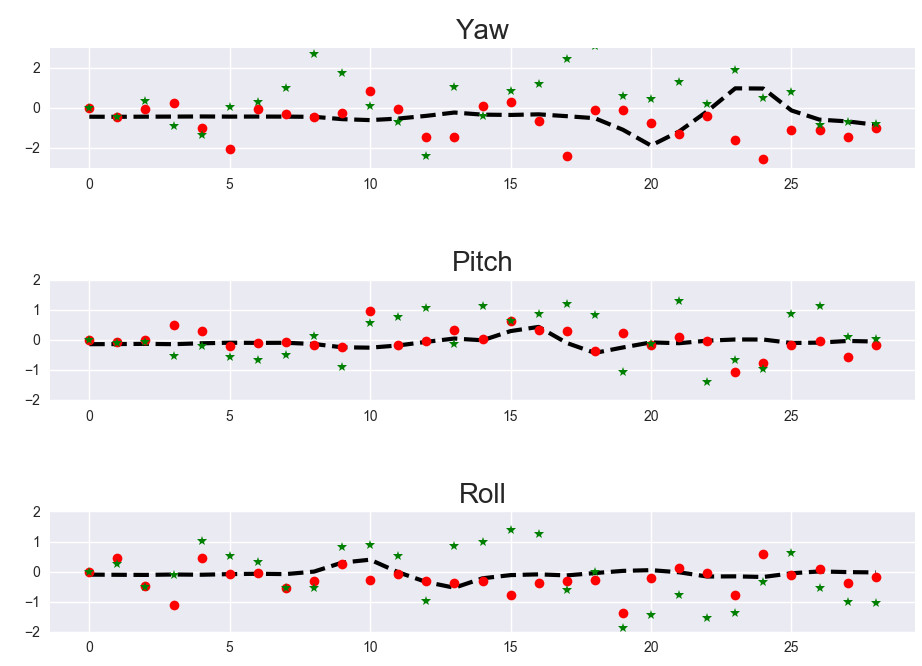
\includegraphics[width=0.47\textwidth]{./content/experiments/figures/noisy-syn-abs-rel-2.jpg}
%   \label{fig:res-noisy-syn-abs-rel}}\hfill
%   \subfigure[The theoretical method with \gls{ransac} optimization]{
%     \includegraphics[width=0.47\textwidth]{./content/experiments/figures/noisy-\gls{ransac}-abs-rel-3.jpg}
%     \label{fig:res-noisy-syn-\gls{ransac}-abs-rel}}
%   \hspace*{\fill}
%   \caption{Absolute and relative rotation obtained from  noisy synthetic data
%     without and with \gls{ransac} optimization. The black line represents the \gls{gt}, the
%     \textcolor{red}{dots} and the \textcolor{green}{stars} represent the
%     absolute and relative predicted rotations, respectively.}
%   \label{fig:noisy-data}
% \end{figure*}

The quantitative results in terms of mean difference ($\mu$) and standard
deviation ($\sigma$) between the predicted rotations and \gls{gt}, for all the
conditions are also shown in the Fig.\,\ref{fig:res-syn}. Note that all the
angles are reported in radians.

%$tabulated in Table.~\ref{tab:tab1}.

% \begin{table}
%   \centering
%   \caption{Mean difference and standard deviation comparison between predicted
%     results and \gls{gt} in radian.}
%   \begin{tabular}{l cc cc cc}
%     \toprule
%     & \multicolumn{2}{c}{Yaw} & \multicolumn{2}{c}{Pitch} &
%                                                             \multicolumn{2}{c}{Roll}\\
%     \midrule
%     & $\mu$ & $\pm \sigma$ &  $\mu$ & $\pm \sigma$ &  $\mu$ & $\pm \sigma$\\
%     \cmidrule{2-3} \cmidrule{4-5} \cmidrule{6-7}

%     Absolute & 0.087 & 0.078 & 0.020 & 0.029 & 0.068 & 0.100 \\
%     Relative & 0.275 & 0.35 & 0.113 & 0.123 & 0.148 & 0.111\\
%     \bottomrule
%   \end{tabular}
%   \label{tab:tab1}
% \end{table}

As illustrated in the obtained results, using the \gls{ransac}
model the outliers are ignored and satisfactory results are achieved.

\subsection{Experiment~2}
\label{sec:exp2}
This section presents the results obtained using real data. The same
experimental setup was used using the \gls{imu} results to create
the \gls{gt} for the vehicle in the world frame.  The original data set
contains 593 recordings which was under-sampled to a sampling rate of 20
frames.  Both absolute and relative methods were ran with \gls{ransac} with the
same parameters than in the previous experiment. The results are presented in
Fig.\,\ref{fig:res-real}.

Even though the difference between the predicted rotation and \gls{gt} using
the real data is higher than for the synthetic measurements the results are
promising and the pose trajectory of the vehicle is respected.


% \begin{table}
%   \centering
%   \caption{Mean difference and standard deviation comparison between predicted
%     results and \gls{gt} in radian on real data.}
%   \begin{tabular}{l cc cc cc}
%     \toprule
%     & \multicolumn{2}{c}{Yaw} & \multicolumn{2}{c}{Pitch} &
%                                                             \multicolumn{2}{c}{Roll}\\
%     \midrule
%     & $\mu$ & $\pm \sigma$ &  $\mu$ & $\pm \sigma$ &  $\mu$ & $\pm \sigma$\\
%     \cmidrule{2-3} \cmidrule{4-5} \cmidrule{6-7}

%     Absolute & 0.23 & 0.22 & 0.27 & 0.18 & 0.15 & 0.19 \\
%     Relative & 0.26 & 0.31 & 0.12 & 0.10 & 0.25 & 0.22\\
%     \bottomrule
%   \end{tabular}
%   \label{tab:tab2}
% \end{table}







%%%Local Variables:
%%% mode: latex
%%% TeX-master: t
%%% End:
